\section{实验设计}
% \textcolor{red}{这一节,主要描述各个模块的功能、接口、逻辑控制方法(状态机控制方法)等。(红字为内容说明,请删除)}
\subsection{单周期改流水线原理}
实验三已完成图中单周期的部分,可以看到,流水线处理器的主要改动,是在每个执行阶段
加入触发器,使得每个周期执行一个阶段,得到的结果送往下一个周期进行执行,同时下一条指
令执行一个阶段,这样能够使指令各阶段并行执行,提升效率。
\begin{figure}[H]
	\centering
	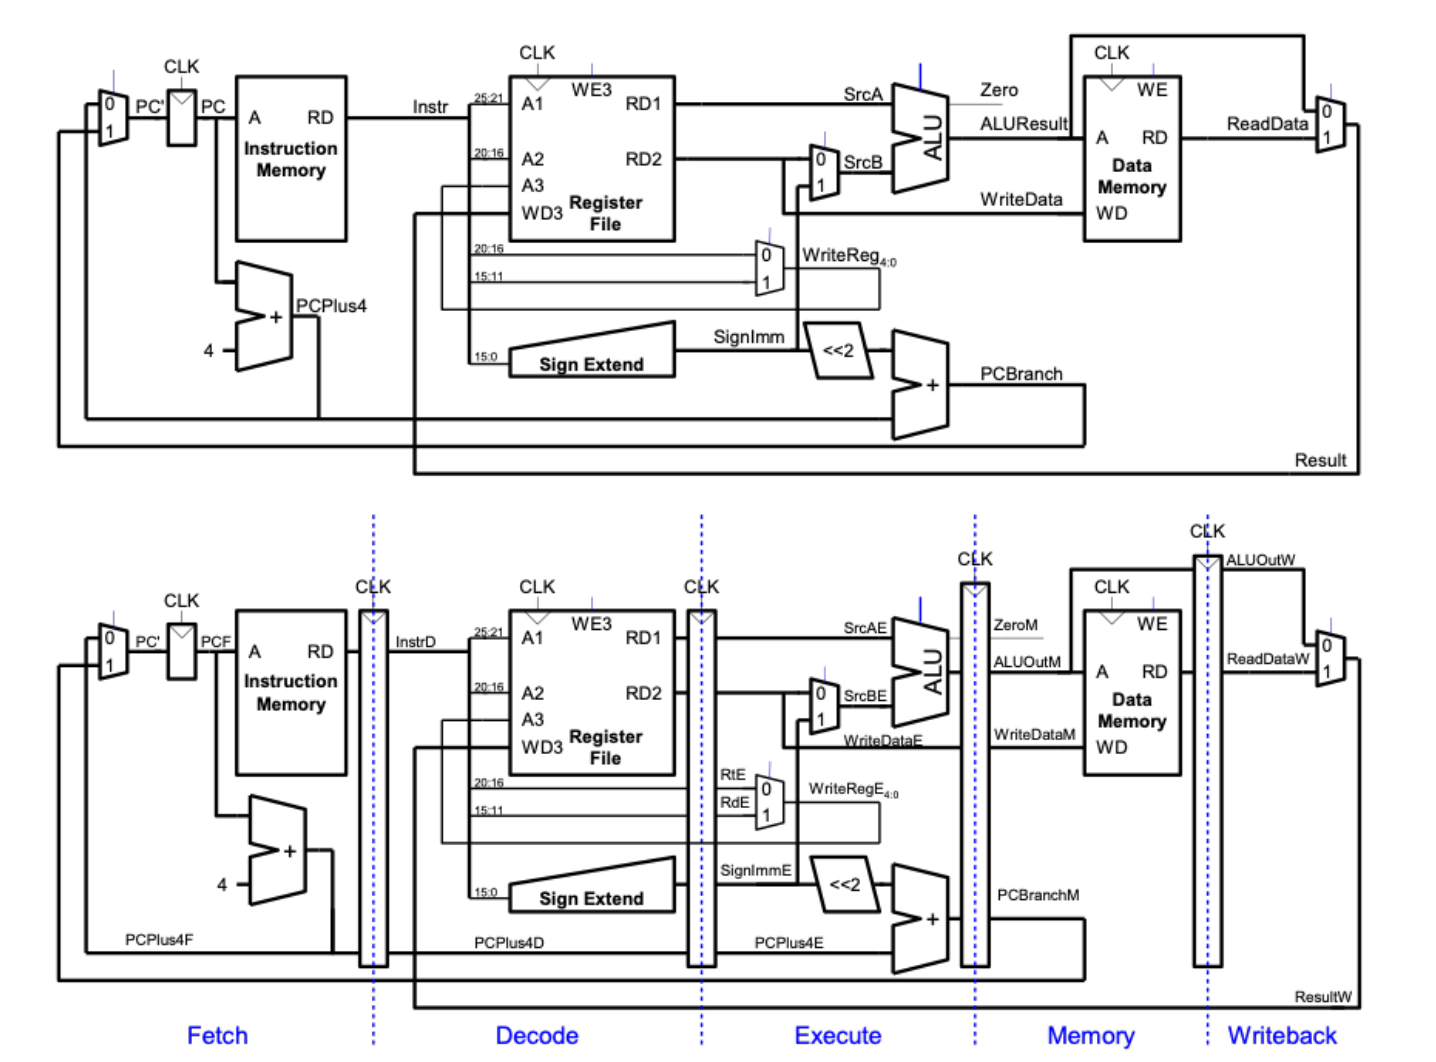
\includegraphics[width=0.75\textwidth]{figure/单周期和流水线比较.png}
	\caption{单周期和流水线比较}
	\label{fig:single_cycle_pipeline}
\end{figure}
可以看到,单周期中写寄存器堆的地址信号 writereg 需要延迟到 writeback 阶段与回写数据
result 一起写回寄存器堆:
\begin{figure}[H]
	\centering
	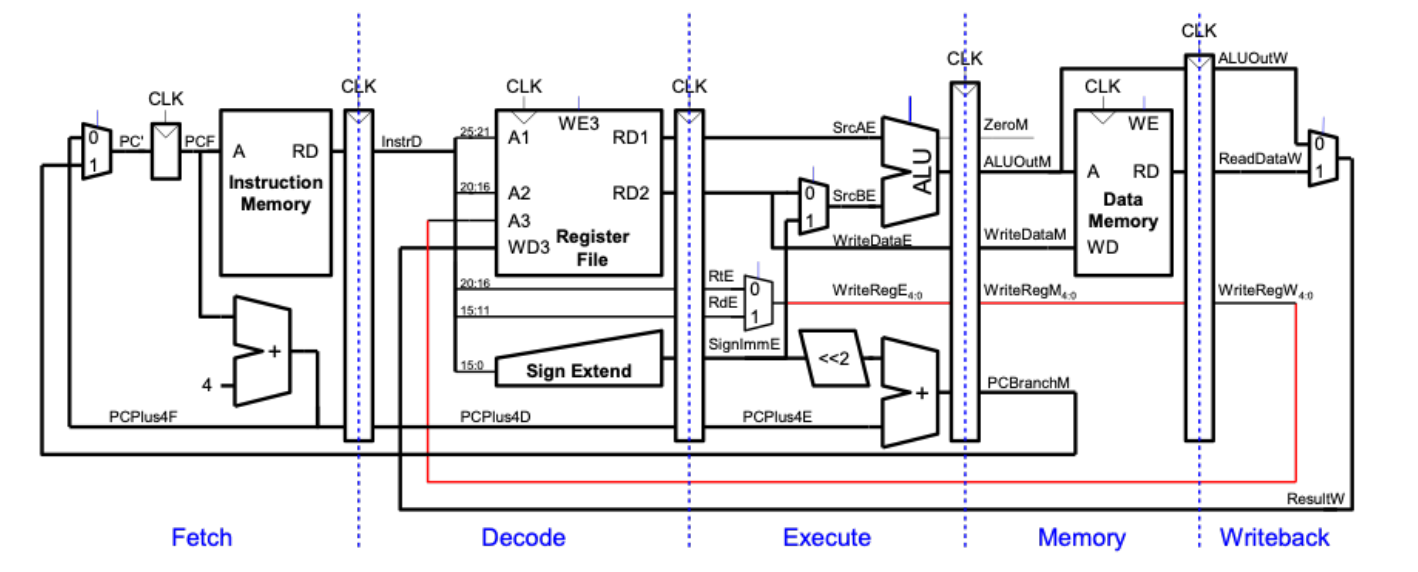
\includegraphics[width=0.75\textwidth]{figure/修改writereg信号.png}
	\caption{修改writereg信号}
	\label{fig:modify_writereg}
\end{figure}
在此基础上,datapath 的基本通路已经形成,下面加入控制器部分。控制器部分与单周期相
同,仍然由 main decoder 和 alu decoder 构成,但由于改为五级流水线后,每一个阶段所需要的控
制信号仅为一部分,控制器产生信号的阶段为译码阶段,产生控制信号后,依次通过触发器传到
下一阶段,若当前阶段需要的信号,则不需要继续传递到下一阶段:
\begin{figure}[H]
	\centering
	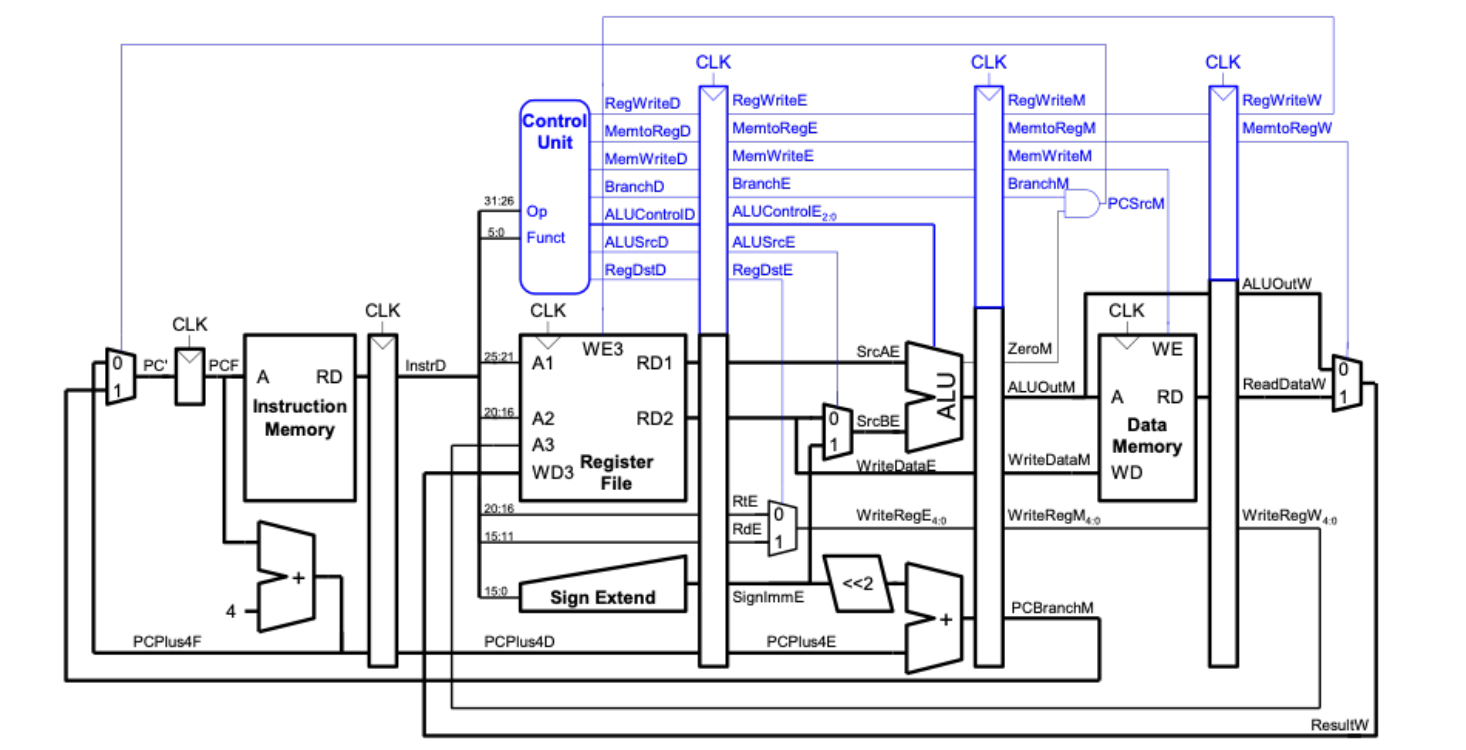
\includegraphics[width=0.75\textwidth]{figure/加入控制器的流水线示意图.png}
	\caption{加入控制器的流水线示意图}
	\label{fig:pipeline_with_controller}
\end{figure}
\subsection{各类型触发器的实现}
实验三中已给出触发器 flopr,作为 PC 使用,此外需要在其基础上实现下列触发器:

(1)flopr:带有 reset 的触发器

(2)floprc:带有 reset 与 clear 的触发器

(3)flopenrc:带有 enable、reset 与 clear 的触发器

flopr 的写法如下:
\begin{lstlisting}[language=Verilog,caption={flopr实现},label={lst:flopr}]

	module flopenr #(parameter WIDTH = 32)
					(input clk,
					 input rst,
					 input en,
					 input [WIDTH-1:0] d,
					 output reg [WIDTH-1:0] q);
		
	always @(posedge clk, posedge rst) begin
		if (rst) begin
			q <= 0;
		end else if (en) begin
			q <= d;
		end
	end
		
	endmodule
		
	
\end{lstlisting}

floprc 的写法如下:
\begin{lstlisting}[language=Verilog,caption={floprc实现},label={lst:floprc}]
module floprc #(parameter WIDTH = 8)
				(input wire clk, rst, clear,
				input wire [WIDTH -1:0] d,
				output reg [WIDTH -1:0] q);

	always @(posedge clk , posedge rst) begin
		if (rst) begin
			q <= 0;
		end else if (clear) begin
			q <= 0;
		end else begin
			q <= d ;
		end
	end

endmodule

\end{lstlisting}
flopenrc 的写法如下:

\begin{lstlisting}[language=Verilog,caption={flopenrc实现},label={lst:flopenrc}]
module flopenrc #(parameter WIDTH = 8)
                 (input wire clk,
                  rst,
                  en,
                  clear,
                  input wire [WIDTH -1:0] d,
                  output reg [WIDTH -1:0] q);
    
    always @(posedge clk) begin
        if (rst) begin
            q <= 0;
        end else if (clear) begin
            q <= 0;
        end else if (en) begin
            /* code */
            q <= d;
        end
    end

endmodule

\end{lstlisting}
\subsection{冒险处理模块}\label{sub:hazard}
在流水线 CPU 中,并不是能够完全实现并行执行,常见的冲突有竞争和冒险。竞争是门电路
两个输入信号同时向相反方向的逻辑电平跳变而导致的现象,本实验不作处理。而对于冒险,在
单周期中由于每条指令执行完毕才会执行下一条指令,并不会遇到冒险问题,而在流水线处理器
中,由于当前指令可能取决于前一条指令的结果,但此时前一条指令并未执行到产生结果的阶段,
这时候,就产生了冒险。本实验设计 hazard 模块处理冒险。

冒险分为:

1. 数据冒险:寄存器中的值还未写回到寄存器堆中,下一条指令已经需要从寄存器堆中读取
数据;

2. 控制冒险:下一条要执行的指令还未确定,就按照 PC 自增顺序执行了本不该执行的指令
(由分支指令引起)。
\subsubsection{功能描述}
1. 数据冒险:
如图 1 中指令,and、or、sub 指令均需要使用 \$s0 中的数据,然而 add 指令在回写阶段才能写
入寄存器堆,此时后续三条指令均已经过或正在执行译码阶段,得到的结果均为错误值。以上就
是数据冒险的特点,数据冒险有以下解决方式:

(1)在编译时插入空指令;

(2)在编译时对指令执行顺序进行重排;

(3)在执行时进行数据前推;

(4)在执行时,暂停处理器当前阶段的执行,等待结果。
\begin{figure}[H]
	\centering
	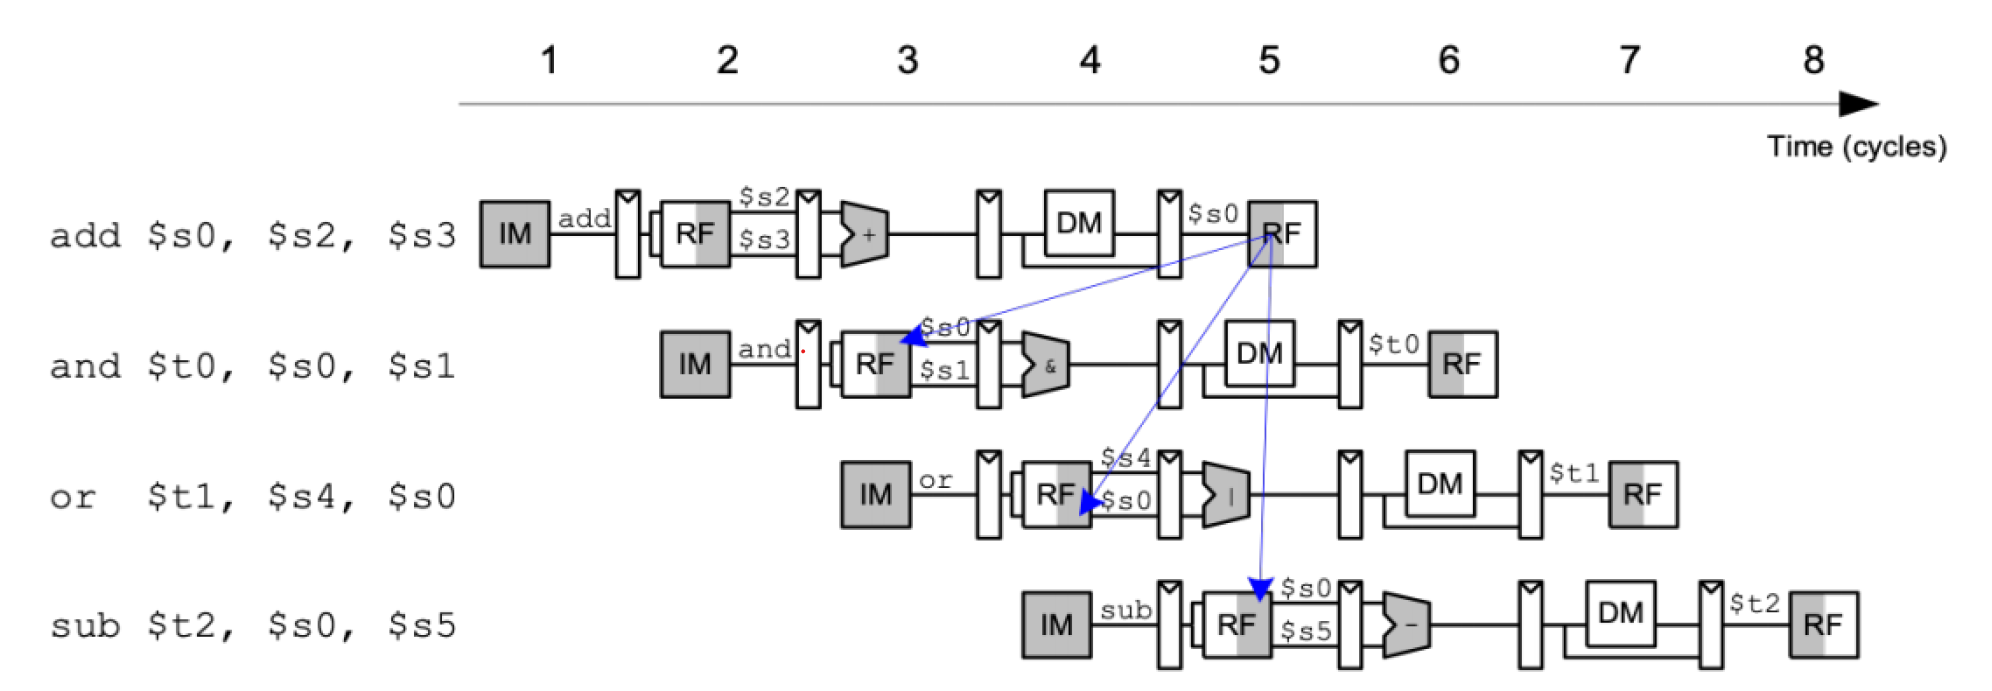
\includegraphics[width=0.75\linewidth]{figure/数据冒险示例.png}
	\caption{数据冒险示例}
	\label{fig:data_hazard}
	\end{figure}

但由于我们未进行指令编译层的处理,因此只需要在运行时 (run time) 进行解决,故采用数
据前推和暂停处理器两种解决方案。

1.1 数据前推

从图 5 所示,add 指令的结果在 execute 阶段已经由 ALU 计算得到,此时可以将 alu 得到的结
果直接推送到下一条指令的 execute 阶段,同理,后续所有的阶段均已有结果,可以向对应的阶段
推送,而不需要等到回写后再进行读取,达到数据前推的目的。
% \textcolor{red}{简单描述实现的功能即可,一句话亦可(红字为内容说明,请删除)}
\begin{figure}[ht]
	\centering
	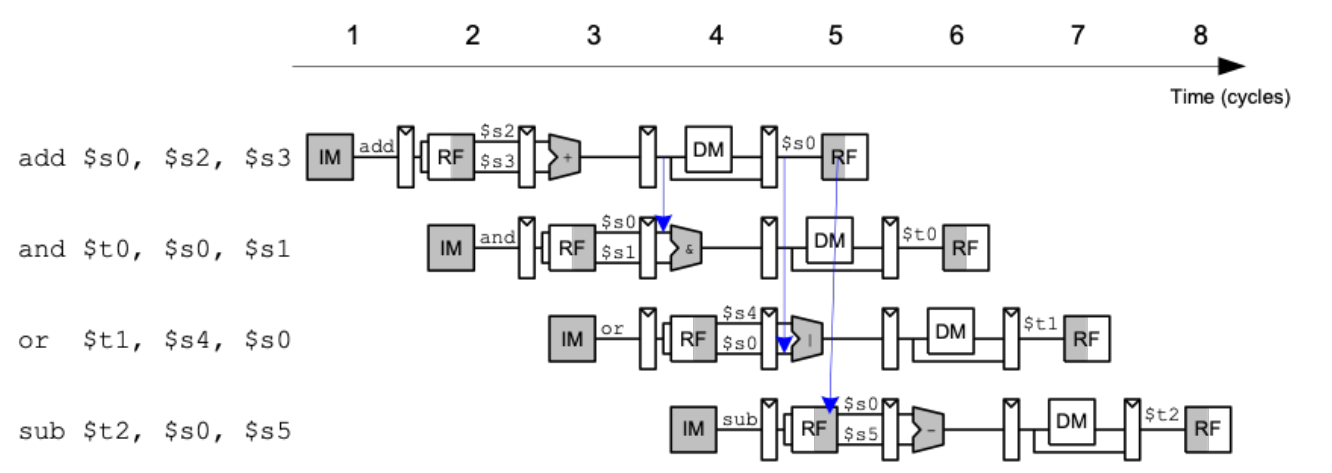
\includegraphics[width=0.75\linewidth]{figure/数据前推示例.png}
	\caption{数据前推示例}
	\label{fig:data_forward_example}
	\end{figure}

从图 5 中可以看到,add 指令的结果在 execute 阶段已经由 ALU 计算得到,此时可以将 alu 得
到的结果直接推送到下一条指令的 execute 阶段,同理,后续所有的阶段均已有结果,可以向对应
的阶段推送,而不需要等到回写后再进行读取,达到数据前推的目的。

数据前推的实现逻辑如下:	
\begin{lstlisting}[language=Verilog,caption={数据前推},label={lst:data_forward}]
	assign forwardAE = ((rsE != 0) && (rsE == writeregM) && regwriteM) ? 2'b10 :
                   ((rsE != 0) && (rsE == writeregW) && regwriteW) ? 2'b01 :
                   2'b00;
	assign forwardBE = ((rtE != 0) && (rtE == writeregM) && regwriteM) ? 2'b10 :
                   ((rtE != 0) && (rtE == writeregW) && regwriteW) ? 2'b01 :
                   2'b00;

\end{lstlisting}

在 execute 阶段需要判断当前输入 ALU 的地址是否与其他指令在此时
执行的阶段要写入寄存器堆的地址相同,如果相同,就需要将其他指令的结果直接通过多路选择
器输入到 ALU 中。

此处需要:

1. 增加 rs,rt 的地址传递到 execute 阶段,并与冒险模块连接;

2. Memory 阶段和 writeback 阶段要写入寄存堆的地址与冒险模块连接;

3. Memory 阶段和 writeback 阶段的寄存器堆写使能信号 regwrite 与冒险模块连接;

4. 根据实现逻辑,将生成的 forward 信号输出,控制 mux3 选择器。

数据通路结构如下:
\begin{figure}[H]
	\centering
	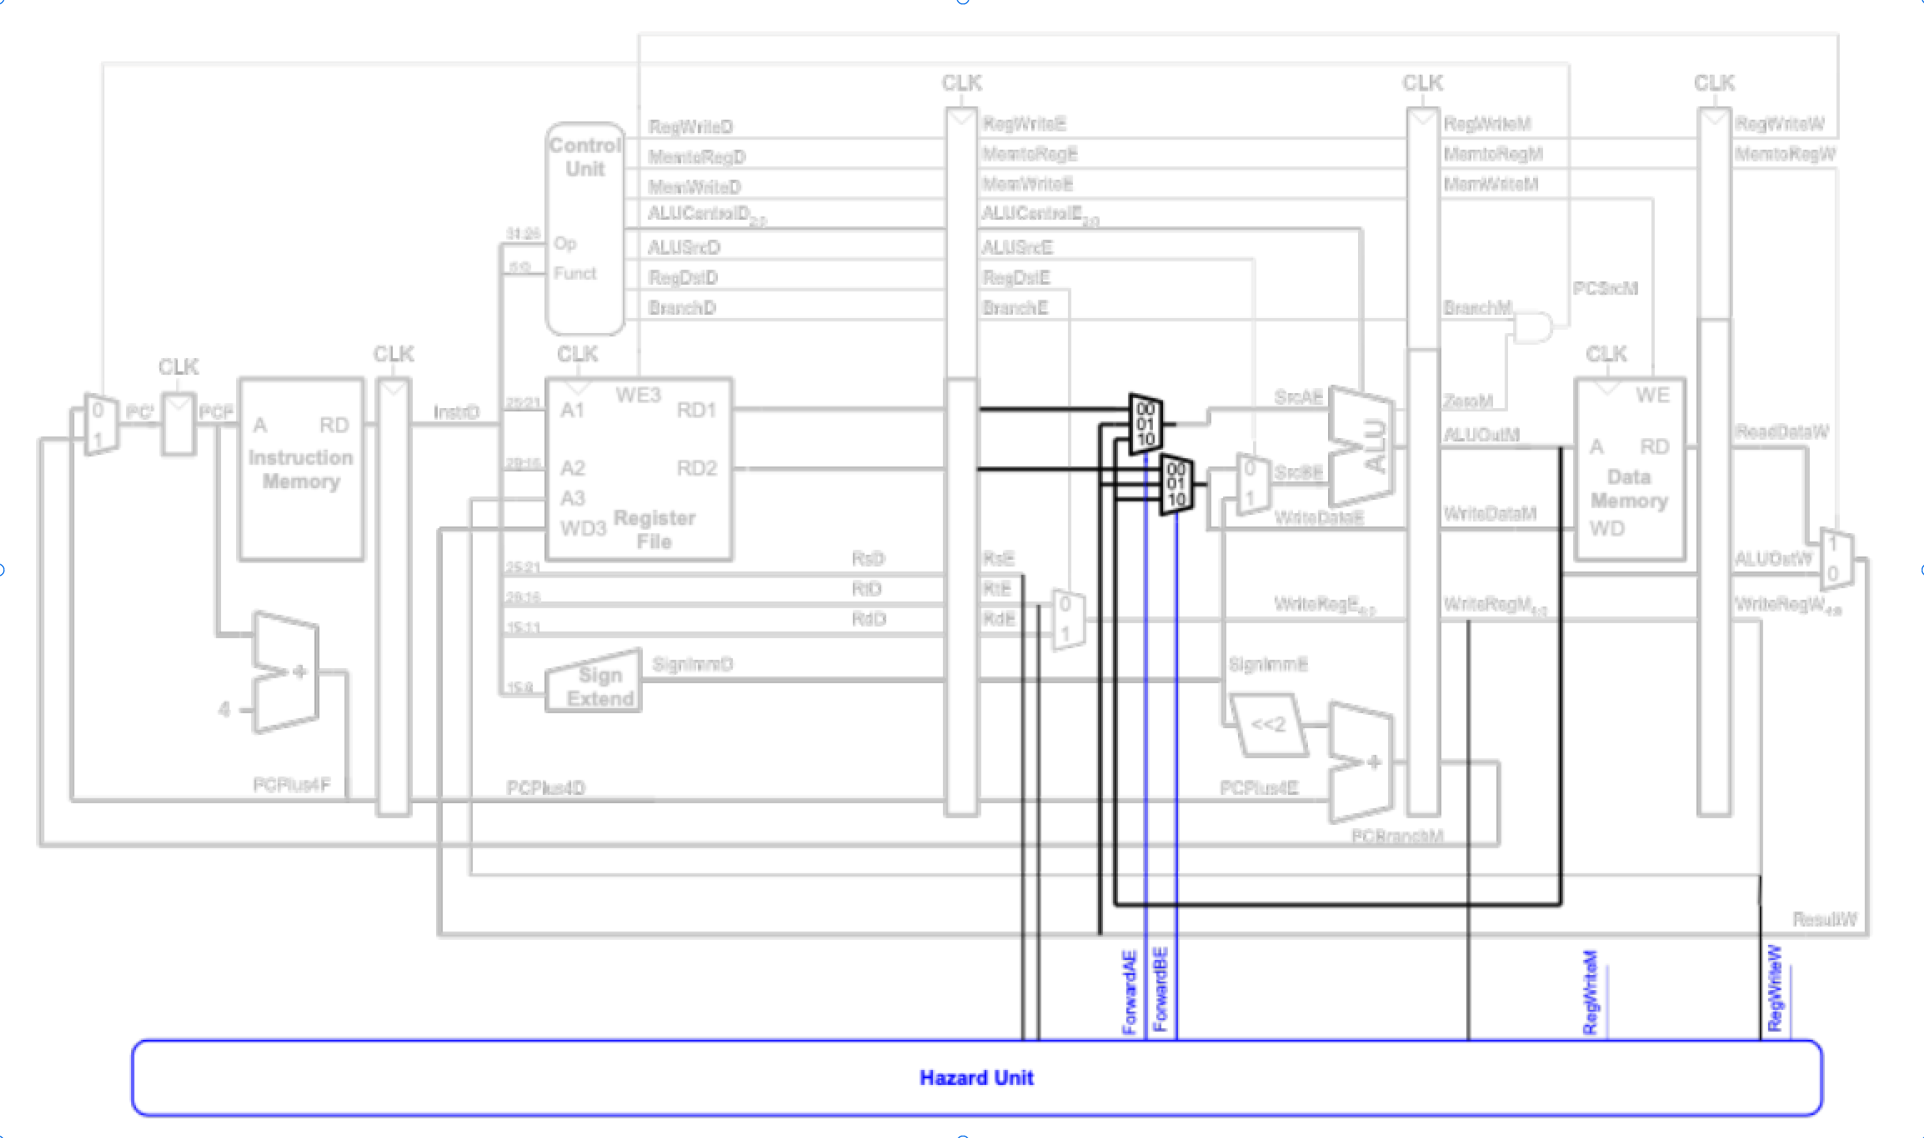
\includegraphics[width=0.75\textwidth]{figure/加入数据前推的数据通路结构.png}
	\caption{加入数据前推的数据通路结构}
	\label{fig:data_forward_data_path}
\end{figure}

1.2 流水线暂停
多数情况下,数据前推能解决很大一部分数据冒险的问题,然而在图中 7,lw 指令在 memory
阶段才能够从数据存储器读取数据,此时 and 指令已经完成 ALU 计算,无法进行数据前推。

如图 8在这种情况下,必须使流水线暂停,等待数据读取后,再前推到 execute 阶段。
\begin{figure}[H]
	\centering
	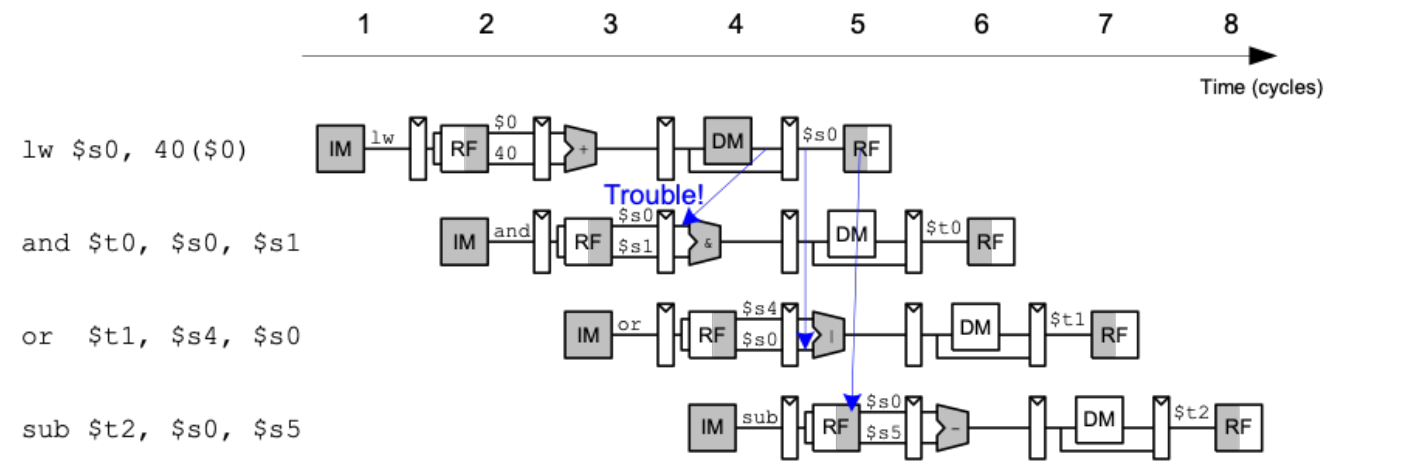
\includegraphics[width=0.75\textwidth]{figure/数据无法前推的情况.png}
	\caption{数据无法前推的情况}
	\label{fig:data_forward_stall}
\end{figure}

\begin{figure}[H]
	\centering
	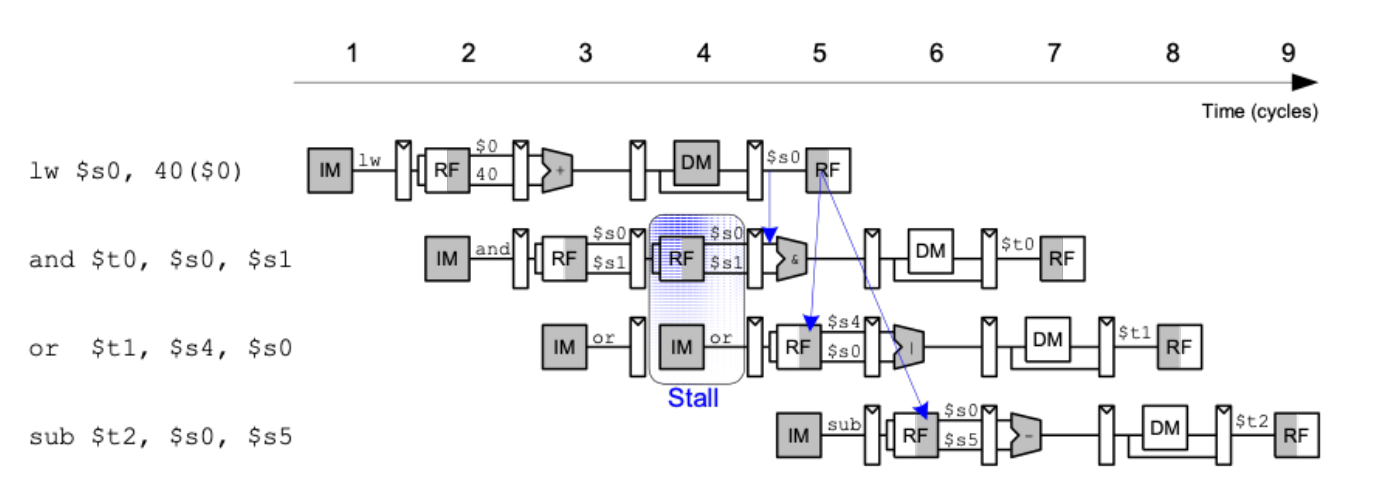
\includegraphics[width=0.75\textwidth]{figure/流水线暂停示例.png}
	\caption{流水线暂停示例}
	\label{fig:data_forward_stall_example}
\end{figure}
流水线暂停的条件是:前一条指令需要对寄存器堆写入 (memturegE=1) 并且写入地址 rtE 与
被当前指令用 (rsD==rtE 或 rtD==rtE)。并且该暂停信号会将后几级流水线全部暂停。注意,流水
线暂停 (decoder 级) 还需要一个附加操作,就是清空 excute 级的信号。因为 lw 下一条指令已经按
照预期接受了流水寄存器 DE 的输出并进行工作。到下面介绍的控制冒险也会用到流水线暂停,
因此将流水线暂停的数据通路和逻辑控制放在控制冒险后介绍。

2. 控制冒险:

控制冒险是分支指令引起的冒险。在五级流水线当中,分支指令在第 4 阶段才能够决定是否
跳转;而此时,前三个阶段已经导致三条指令进入流水线开始执行,这时需要将这三条指令产生
的影响全部清除。
\begin{figure}[H]
	\centering
	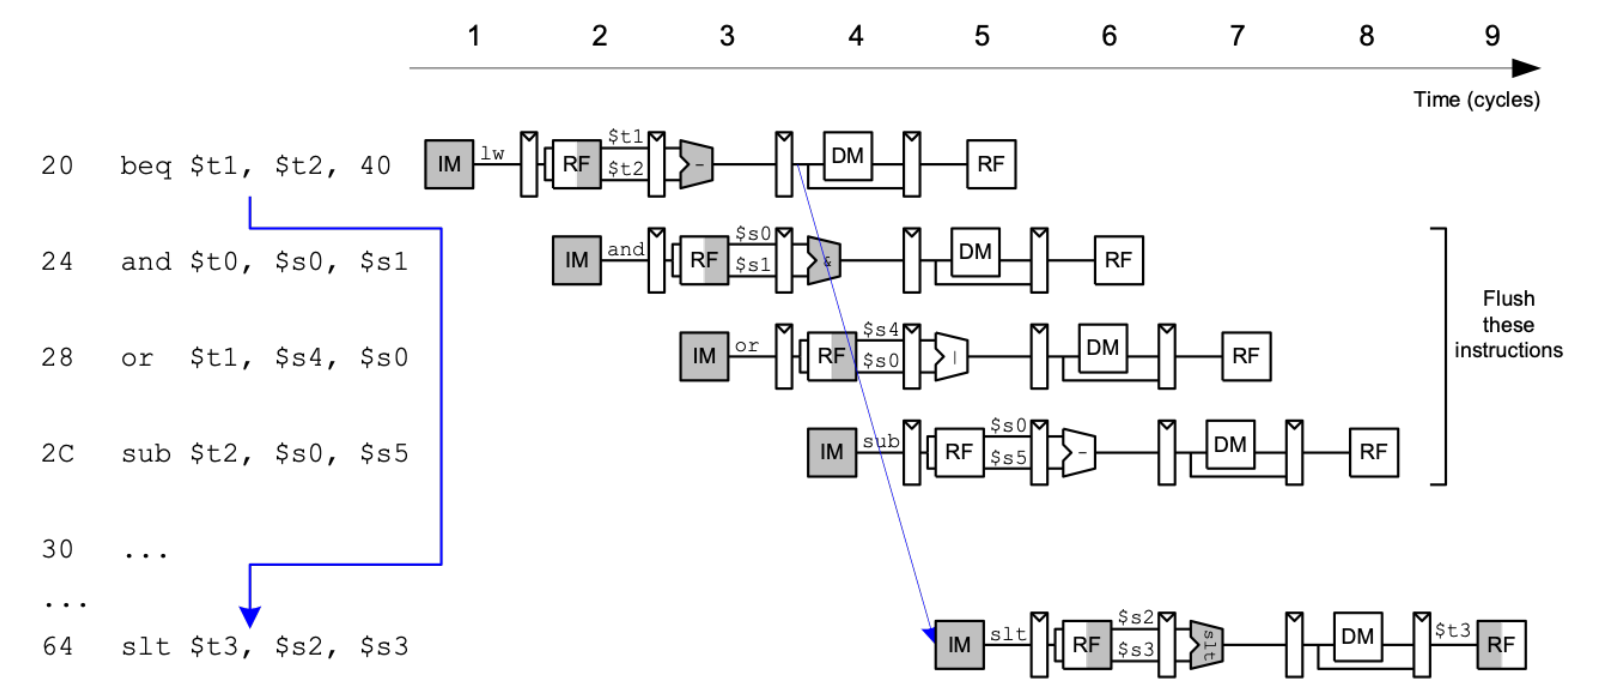
\includegraphics[width=0.75\textwidth]{figure/控制冒险示例.png}
	\caption{控制冒险示例}
	\label{fig:control_hazard}
\end{figure}
将分支指令的判断提前至 decode 阶段,此时能够减少两条指令的执行;
\begin{figure}[H]
	\centering
	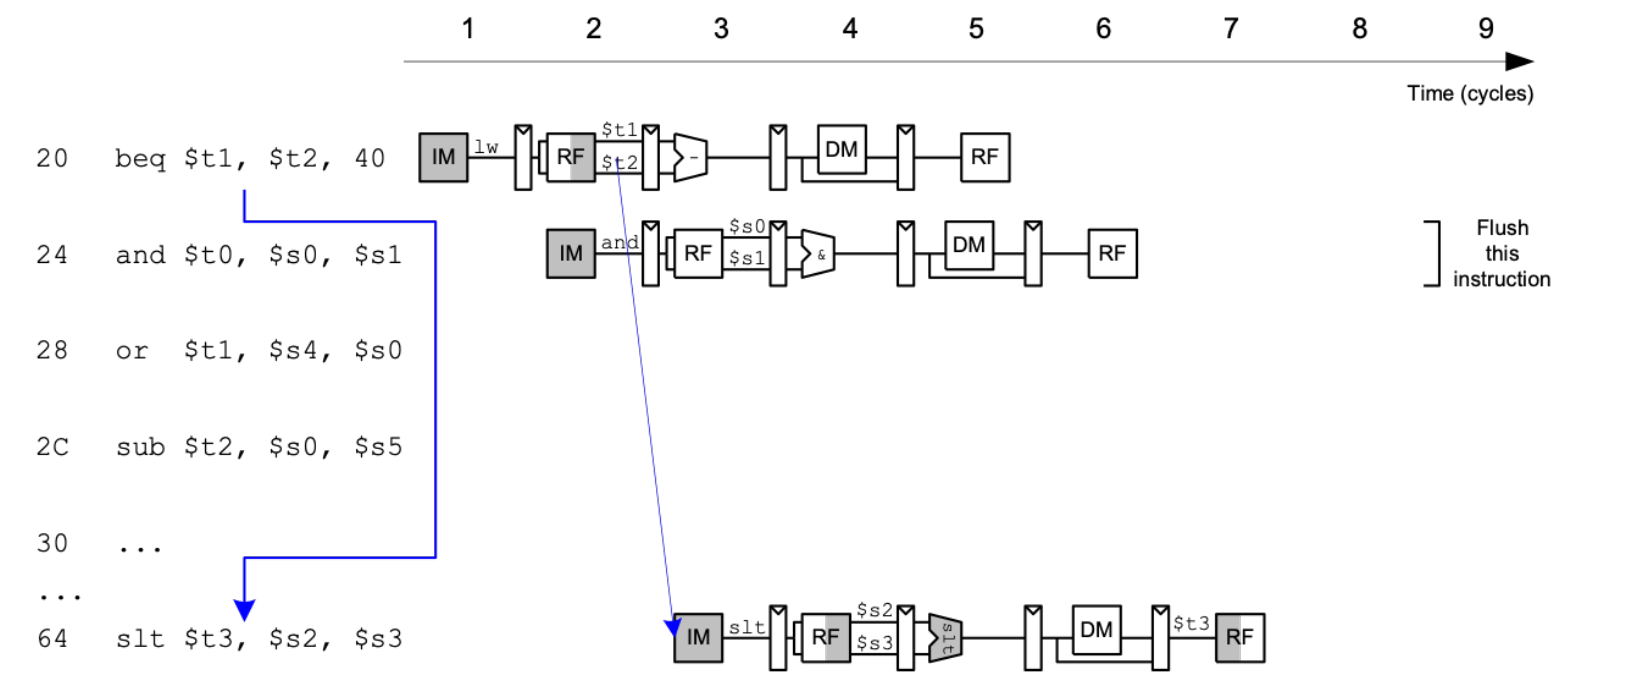
\includegraphics[width=0.75\textwidth]{figure/提前判断分支.png}
	\caption{提前判断分支}
	\label{fig:control_hazard_forward}
\end{figure}
在 regfile 输出后添加一个判断相等的模块,即可提前判断 beq:
\begin{figure}[H]
	\centering
	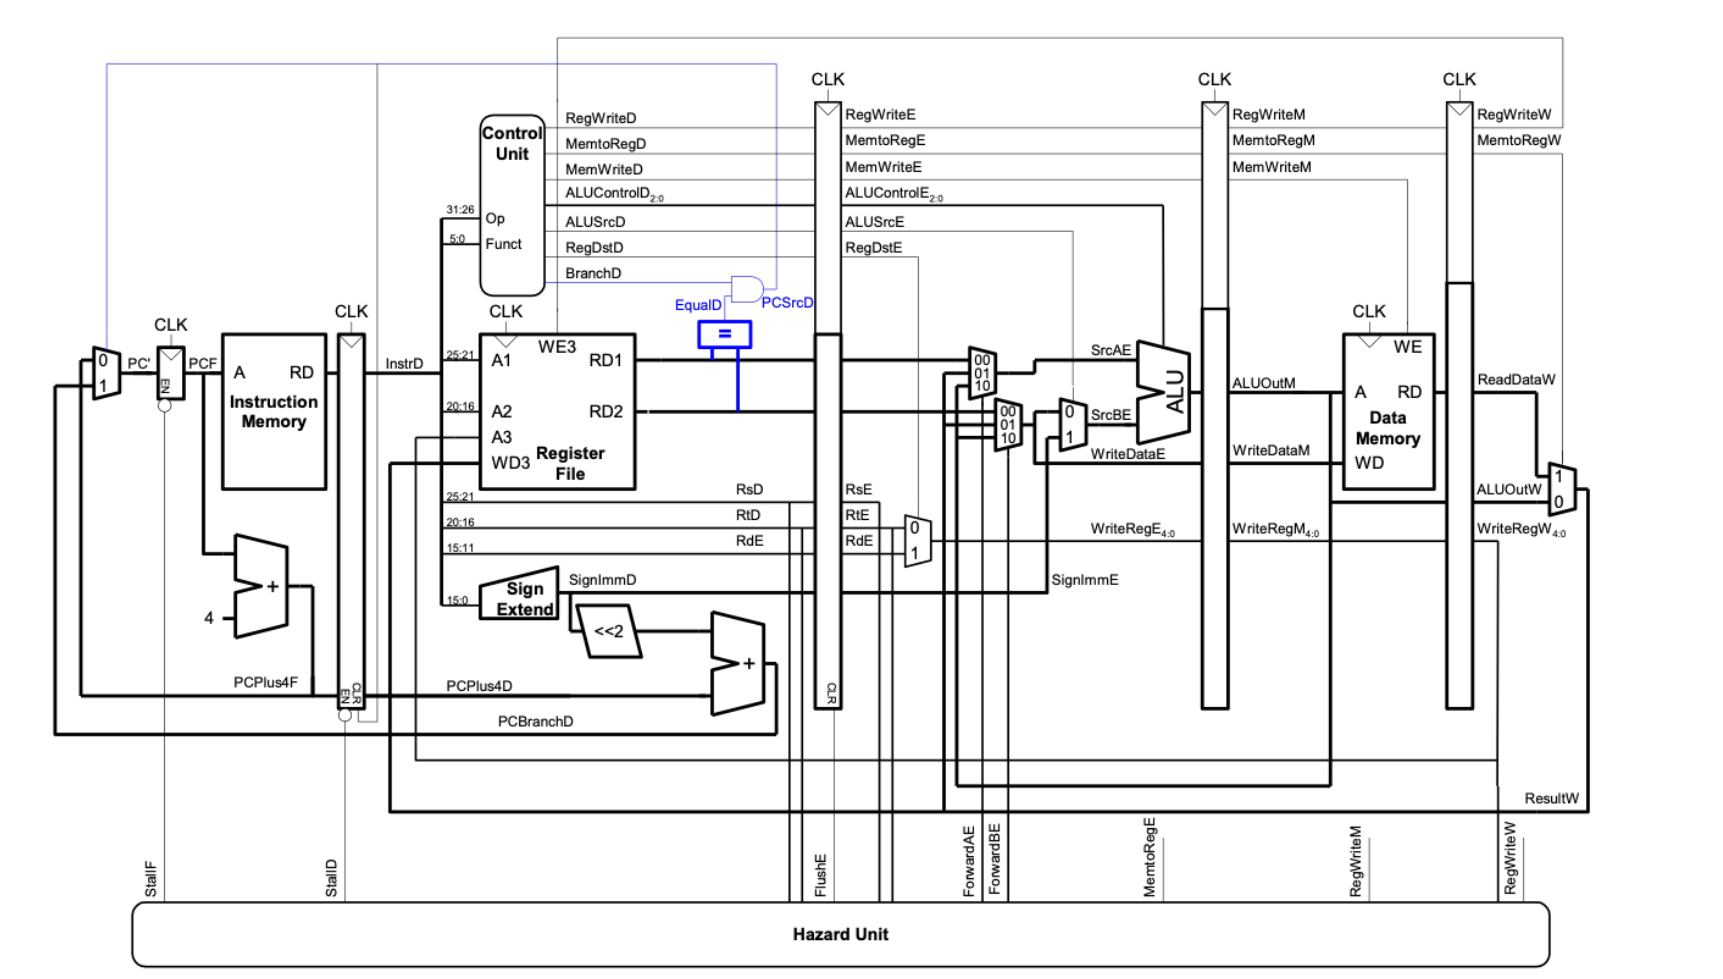
\includegraphics[width=0.75\textwidth]{figure/提前判断分支的实现.png}
	\caption{提前判断分支的实现}
	\label{fig:control_hazard_forward_implementation}
\end{figure}
此时又产生了数据冲突问题,需要增加数据前推和流水线暂停模块;
\begin{figure}[H]
	\centering
	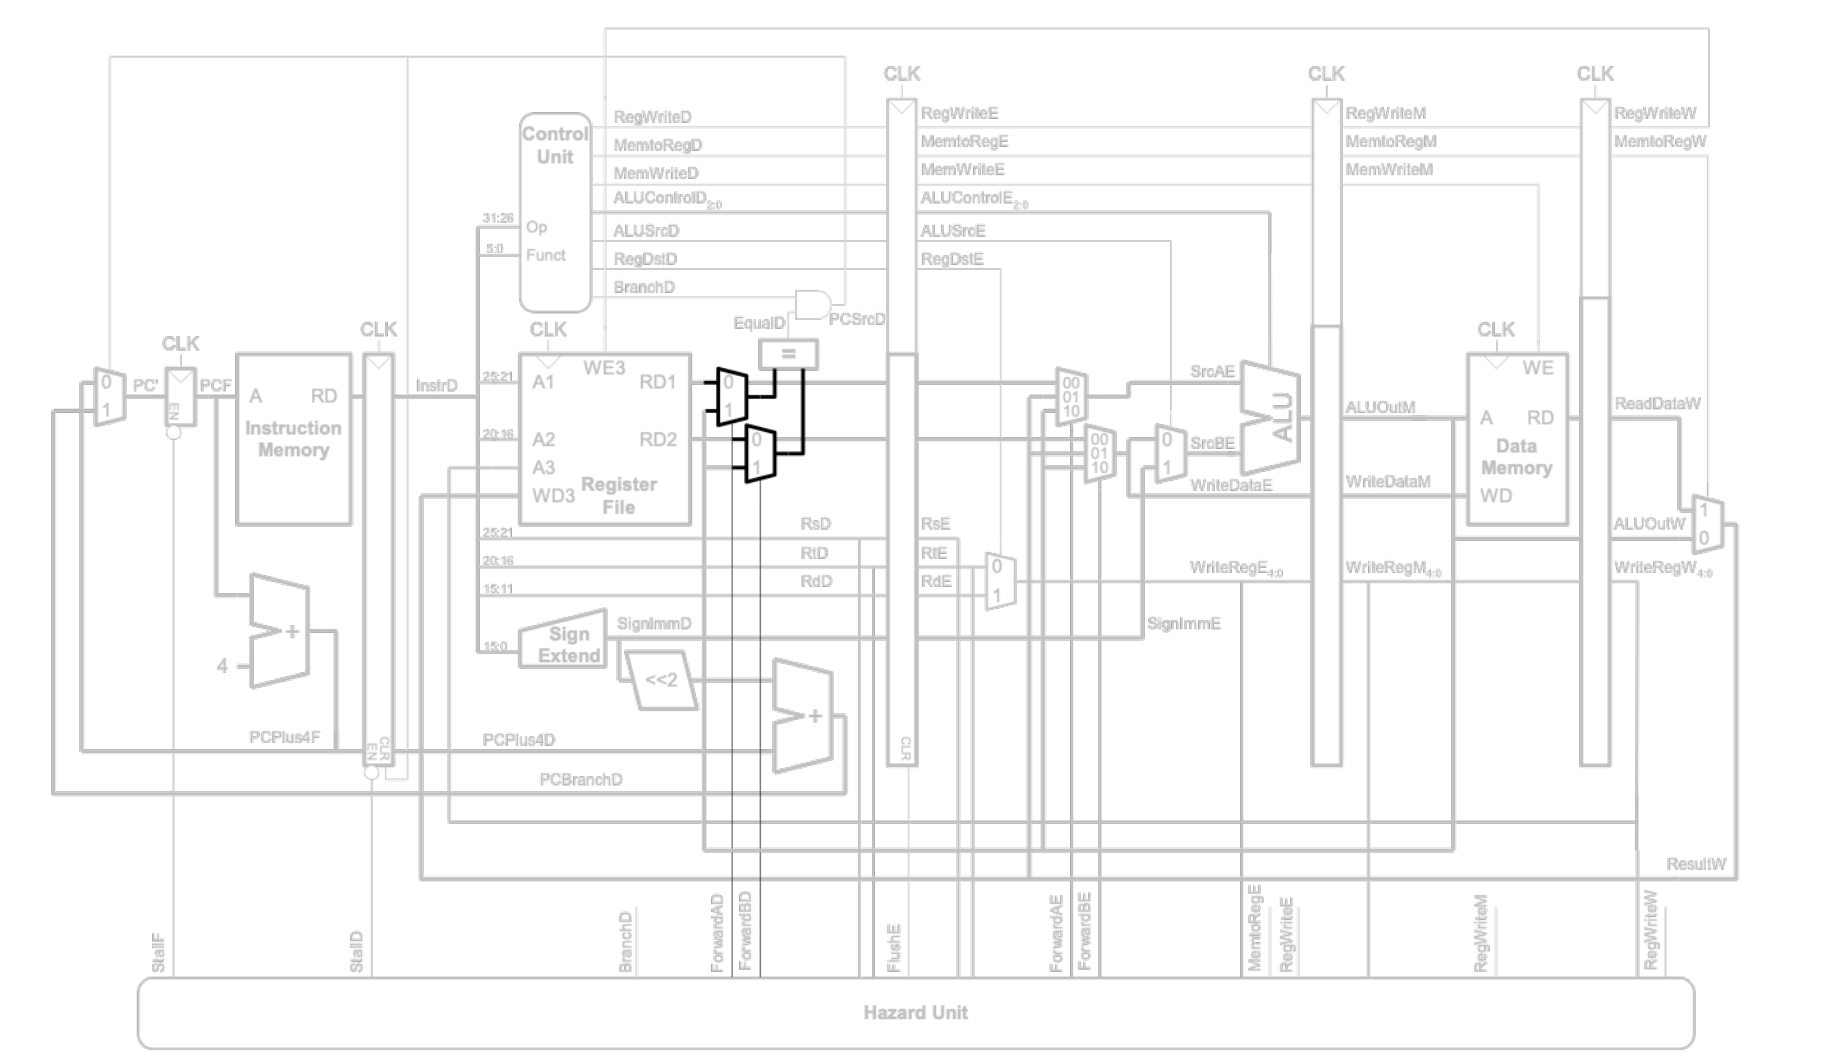
\includegraphics[width=0.75\textwidth]{figure/解决控制冒险的数据通路.png}
	\caption{解决控制冒险的数据通路}
	\label{fig:control_hazard_data_path}
\end{figure}
控制冒险的逻辑控制如下:
\begin{lstlisting}[language=Verilog,caption={控制冒险逻辑控制},label={lst:control_hazard_logic}]
	assign forwardAD = ((rsD != 0) && (rsD == writeregM) && regwriteM);
	assign forwardBD = ((rtD != 0) && (rtD == writeregM) && regwriteM);
	
	// --------------------------------
	// stall
	wire lwstall;
	//stallF, stallD, flushE;
	wire branchstall;
	assign lwstall = ((rsD == rtE) || (rtD == rtE)) && memtoregE; // . 判断 decode 阶段 rs 或 rt 的地址是否是 lw 指令要写入的地址;
	assign branchstall = branchD && regwriteE && 
						   (writeregE == rsD || writeregE == rtD) ||
						   branchD && memtoregM &&
						   (writeregM == rsD || writeregM == rtD);
	
	assign stallF = lwstall || branchstall;
	assign stallD = lwstall || branchstall;
	assign flushE = lwstall || branchstall;
\end{lstlisting}
\subsubsection{接口定义}
% \textcolor{red}{接口定义请使用表格,需要包括\textbf{接口信号名、方向、宽度、含义}(红字为内容说明,请删除)}

% \begin{table}[htp]
% \caption{接口定义模版}\label{tab:signaldef}
% \begin{center}
% 	\begin{tabular}{|l|l|l|p{6cm}|}
% 	\hline
% 	\textbf{信号名} & \textbf{方向} & \textbf{位宽} & \textbf{功能描述}\\ \hline \hline
% 	valid			& Output& 1-bit & If CPU stopped or any exception happens, valid signal is set to 0.\\ 
% 	\hline
% 	\end{tabular}
% \end{center}
% \end{table}

\begin{table}[H]
	\caption{接口定义}\label{tab:signaldef}
	\begin{center}
	\begin{tabular}{lllp{6cm}}
	\hline
	\textbf{信号名} & \textbf{方向} & \textbf{位宽} & \textbf{功能描述} \\ \hline \hline
	rst & Input & 1-bit & 重置信号 \\ \hline
	rsD & Input & 5-bit & decoder 阶段的 rs 号码 \\ \hline
	rtD & Input & 5-bit & decoder 阶段的 rt 号码 \\ \hline
	rsE & Input & 5-bit & execute 阶段的 rs 号码 \\ \hline
	rtE & Input & 5-bit & execute 阶段的 rt 号码 \\ \hline
	regwriteE & Input & 1-bit & execute 阶段的寄存器写使能 \\ \hline
	regwriteM & Input & 1-bit & memory access 阶段的寄存器写使能 \\ \hline
	regwriteW & Input & 1-bit & writeback 阶段的寄存器写使能 \\ \hline
	memtoregE & Input & 1-bit & execute 阶段指令是否需要将数据读写至寄存器 \\ \hline
	memtoregM & Input & 1-bit & memory 阶段指令是否需要将数据读写至寄存器 \\ \hline
	branchD & Input & 1-bit & decoder 阶段判断是否为分支指令 \\ \hline
	writeregE & Input & 5-bit & execute 阶段的寄存器写号码 \\ \hline
	writeregM & Input & 5-bit & memory 阶段的寄存器写号码 \\ \hline
	writeregW & Input & 5-bit & writeback 阶段的寄存器写号码 \\ \hline
	forwardAE & Output & 2-bit & execute 阶段由 mux3 选择 SrcA \\ \hline
	forwardBE & Output & 2-bit & execute 阶段由 mux3 选择 SrcB \\ \hline
	forwardAD & Output & 2-bit & decoder 阶段由 mux3 选择 SrcA \\ \hline
	forwardBD & Output & 2-bit & decoder 阶段由 mux3 选择 SrcB \\ \hline
	stallF & Output & 1-bit & fetch 阶段停滞 \\ \hline
	stallD & Output & 1-bit & decoder 阶段停滞 \\ \hline
	flushE & Output & 1-bit & 清空 execute 阶段状态 \\ \hline
	\end{tabular}
	\end{center}
	\end{table}